\documentclass[titlepage, 13px, a4paper]{article}

\usepackage[utf8]{inputenc}

\usepackage[T1]{fontenc}
\usepackage{fontawesome}
\usepackage{eurosym}

\usepackage[french]{babel}

\usepackage{fancyhdr}
\usepackage{graphicx}
\usepackage[left=4.5cm,right=4cm,top=4.5cm, textheight=17cm]{geometry}
\usepackage{wrapfig}

\usepackage{eso-pic}
\usepackage{transparent}

\usepackage{hyperref}
\usepackage{setspace}

\usepackage{titletoc}
\usepackage{titlesec}

\usepackage{stackengine,xcolor}
\usepackage{enumerate}

\titleclass{\part}{top}
\titleformat{\part}[display]
  {\normalfont\huge\bfseries}{\centering\partname\ \thepart}{20pt}{\Huge\centering}
\titlespacing*{\part}{0pt}{50pt}{40pt}
\titleclass{\chapter}{straight}
\titleformat{\chapter}[display]
  {\normalfont\huge\bfseries}{\chaptertitlename\ \thechapter}{20pt}{\Huge}
\titlespacing*{\chapter} {0pt}{50pt}{40pt}

%\usepackage{titlesec}
%\titleformat{\part}[display]
  %{\normalfont\bfseries}{}{0pt}{\Large\bfseries}

\newcommand\BackgroundPic{%
	\put(0,-50){%
		\parbox[b][\paperheight]{\paperwidth}{%
			%\vfill
			\centering
			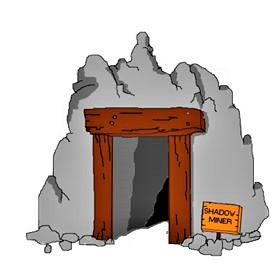
\includegraphics[%
			keepaspectratio]{../images/icone.jpg}%
			\vfill
		}
	}
}

\fboxrule=2pt
\newcommand\cincludegraphics[2][]{%
  \setbox0=\hbox{\includegraphics[#1]{#2}}%
  \abovebaseline[-.5\ht0]{\includegraphics[#1]{#2}}}

  
\renewcommand{\baselinestretch}{1}
\renewcommand{\partname}{}


\title{\textbf{{\Huge Manuel d'utilisation}}}
\author{
	\\
	\bsc{{\LARGE \bf ShadowMiner}} \\ \\ \\
	\bsc{{\LARGE \bf par ACCEr}} \\ \\
}
\date{{\LARGE \today}}

\pagestyle{fancy}
%\fancyfoot[L]{
\includegraphics{../images/ShadowMiners_logo_mini.png}} %50x33
\fancyfoot[L]{\cincludegraphics[scale=0.1]{../images/ShadowMiners_logo.png}} %50x33
\fancyfoot[R]{STRASBOURG 2022}
\fancyhead[R]{ACCEr}
\fancyhead[L]{Manuel d'utilisation}

\setcounter{tocdepth}{3}

\begin{document}
\AddToShipoutPicture*{\BackgroundPic}

\maketitle
\tableofcontents

\newpage 
\part{Introduction} 


\newpage 
\part{Présentation du projet}  
\section{Contexte} 
\paragraph{} \hspace{0pt} 
Ce projet est réalisé dans le cadre de la mise en oeuvre des connaissances acquises 
lors des cours de TD et TP informatiques et nous permet de renforcer et d’approfondir nos apprentissages.   

\section{Objectif} 
\paragraph{} \hspace{0pt} 
Le  premier  objectif de ce projet est de réaliser un jeu vidéo en équipe de quatre pendant les cinq mois à venir 
et représente un première expérience des travaux en équipe qui jalonneront notre future vie professionnelle. 
\section{L'équipe} 
\paragraph{} \hspace{0pt} 
Ce projet est fait par le groupe ACCEr composé d’ Antoine Claudel, de Cédric Farinazzo, 
de Clément Languerre et d’Edgar Grizzi. 
\section{La démarche} 
\paragraph{} \hspace{0pt} 
Dans une premier temps, nous expliquerons l’origine du projet en partant de l’idée principale 
et des réflexions qui ont suivies.  

Dans un second temps nous présenterons  le principe du jeu ainsi que les objectifs que nous nous 
sommes fixés sur le mode solo et sur le mode multijoueurs. 
Nous soulignerons également ce que ce projet pourra nous apporter d’un point de vue individuel 
ou en tant que groupe.
  
Nous verrons  ensuite, nos sources d’inspirations en tant qu'amateurs de jeux vidéos, 
qui ont déterminé la nature de ce projet et la conception du jeu en mode solo et en mode multi-joueur.  

Enfin nous aborderons la partie organisation de notre projet, la partie technique 
qui mentionne les logiciels utilisés, les aspects économiques, la répartition des tâches et le planning. 
Nous vous expliquerons le commencement de ce projet, tout d'abord avec l'idée principale,  
ensuite la réflexion que nous avons eue sur cette idée, ce qui fera l'origine du projet. 

\newpage

\part{Origine et nature du projet}
\section{De l'idée vers le projet}
\paragraph{} \hspace{0pt}
Tout d'abord nous nous sommes dit "Réfléchissons chacun de notre côté puis  concertons nous pendant les vacances.".
Le 1er Janvier pour bien commencer l'année, Cédric nous a envoyé un message pour faire le point. A la fin de notre discussion, deux idées sont ressorties : 
Une idée de battle royal ou une idée de jeu d'horreur avec un monstre qui poursuit un homme dans une mine.
Après un vote, nous avons choisi l'idée de la mine qui nous parut  la plus originale car les jeux de battle royal sont trop  à la mode en ce moment.

\section{Nom et concept du jeu : Shadow Miner}
\paragraph{} \hspace{0pt}
Nous avons donc décidé de le baptiser "Shadow Miner" car l’histoire du jeu se passe dans une mine.
Le jeu se déroulera à la première personne (vision subjective).
Nous avons pensé à un mode solo et un mode multijoueurs.

\section{Mode solo}
\paragraph{} \hspace{0pt}
Pour le mode solo, nous avons deux histoires possibles :
{\begin{enumerate}
	\item Un groupe de personnes, habitant dans le village à proximité de la mine désaffectée, 
		a entendu des bruits provenant de la mine. Le groupe décide de descendre dans la mine 
		pour aller voir ce qu’il se passe. Lors de leur descente via l’ascenseur, 
		les câbles de ce dernier sont coupés et l’ascenseur descend au fond de la mine. 
		Les survivants tentent alors de remonter à pied dans ce dédale. Ils rencontreront des pièges 
		et un mineur sombre qui fera tout pour les empêcher de remonter à la surface.
		L’utilisateur incarnera un des survivants tentant de rejoindre la surface dans une succession de niveaux plus difficiles les uns que les autres. \newpage
	
	\item Un mineur descend tôt le matin dans les derniers sous-sols de la mine, là où l’oxygène se fait rare. 
		Un mineur fou (le Shadow Miner) coupe les câbles de l’ascenseur. 
		Le mineur veut alors rejoindre la surface. Le Shadow Miner va alors vouloir l’en empêcher.
		L’utilisateur incarne alors le mineur. \\
\end{enumerate}}

\section{Mode multijoueurs}
\paragraph{} \hspace{0pt}
Dans ce mode, nous avons pensé qu'un joueur serait le Shadow Miner 
et devrait tuer les deux autres joueurs qui incarneront deux mineurs voulant rejoindre la surface. 
Un des mineurs pourra s’enlever la vie et devenir un esprit de la mine 
qui contrôle les cloisons de la mine (porte, mur, gouffre) pour aider l’autre mineur.

\section{Gameplay}
\paragraph{} \hspace{0pt}
Le joueur, autant en mode solo qu'en mode multijoueurs, sera ralenti dans sa progression 
à cause des pièges et d'autres animations (éboulements, piques, ...)  qui pourront le bloquer, le blesser, voire le tuer. 
Ces pièges s’appliqueront aussi bien au mineur qu'au shadow miner.
Le joueur progressera de niveaux en niveaux avec des options de sauvegarde.
\\
Chaque niveau sera composé d’un point de départ et d'un checkpoint qui représentera la fin du niveau.
Si le joueur parvient au checkpoint, alors il pourra passer au niveau suivant.
\\
Sinon il devra recommencer le niveau.
\\
Le joueur sera équipé par défaut d'une torche et d'une pioche. Les torches seront indispensables puisqu'elles permettront de voir dans l'obscurité.
Les pioches permettront de se défendre contre de potentielles créatures ou de creuser pour s'échapper.
Ces équipements pourront être perdus au cours de l'aventure.


\newpage

\part{Apports collectifs et personnels}

\paragraph{} \hspace{0pt} \\
Les intérêts du travail en équipe sont communs à tous les domaines :
\begin{itemize}
	\item l'efficacité est multipliée (par 4 ici),
	\item les idées sont plus nombreuses et variées,
	\item le projet peut être plus ambitieux grâce à l'entraide et la répartition des tâches et surtout la motivation est toujours présente, chacun veut donner le meilleur de soi-même. 
\end{itemize}

\paragraph{} \hspace{0pt} \\
Outre la satisfaction de réaliser entièrement un jeu vidéo, ce projet nous apporte de l'expérience, développe notre esprit d'équipe et nous entraîne à tenir les objectifs que nous nous donnons dans un temps restreint. 

\newpage

\part{Inspiration}
\section{Du mode solo}
\paragraph{} \hspace{0pt} \\
Le jeu possède un mode solo et un mode multijoueurs, inspiré de jeux différents. 
Le mode solo est un "survival horror" imaginé à partir des jeux d'horreur du moment, 
en particulier "Outlast" et "Alien: Isolation" sortis en 2013 et 2014. 
\\
Le principe est de s'enfuir d'une mine en progressant dans une aventure guidée 
avec des «screamers» (moments de frissons/ frayeurs) prédéfinis et un scénario. 
Si le joueur n'est pas assez réactif, il peut mourir.
\\
Le terme "survival horror" est utilisé pour la première fois en 1996 lors de la sortie 
de Resident Evil. Parmi les "survivals horror" les plus connus, il y a "Outlast" qui 
nous a inspirés mais aussi "Until Dawn" et "Alien : Isolation". 
\\
Dans "Outlast", le joueur prend le contrôle d'un journaliste qui enquête sur un asile psychiatrique; 
"Until Dawn" raconte l'histoire d'un groupe de jeunes qui se rend dans un châlet 
en montagne pour passer les vacances. Le point fort de ce jeu réside dans son mode 
de jeu à la Heavy Rain ou Beyond Two Souls, c'est un film interactif dont l'histoire 
change radicalement en fonction des choix de l'utilisateur. 
\\
"Alien : Isolation", qui se déroule quatorze ans après les évènements du film "Alien, le huitième passager" 
et l'histoire est respectée dans les moindres détails. 

\newpage
\section{Du mode multijoueurs}
\paragraph{} \hspace{0pt} \\
Le mode multijoueurs est un "2 vs 1" dans le même genre que "Dead Realm", "Evolve" 
ou même "Mario Chase" dans Nintendo Land sur Wii U. 
\\
Dans "Dead Realm", 3 joueurs se retrouvent dans un décor effrayant (vieux manoir, jardin de nuit,...) enfermés 
avec un monstre terrifiant (loup garou, bébé tueur, clown) qui peut les transformer 
en spectre et s'en faire des alliés pour éliminer tous les survivants. 
\\
Dans "Evolve", 4 joueurs avec des compétences spécifiques se regroupent pour capturer 
une bête mais elle devient plus forte au fil du temps et au final le chassé devient le chasseur. 
\\
"Mario Chase" est un mini jeux de cache-cache ou un joueur possède une mini map 
avec la position de chaque joueur et doit réussir à ne pas se faire attraper par les autres. 
\\
Dans notre projet , "Shadow Miner", un joueur incarne le mineur fou de la mine et les 2 autres 
joueurs tentent de lui échapper. Parmi les 2 mineurs il peut y avoir un architecte (ou chef mineur ou encore esprit de la mine) 
qui connaît parfaitement les moindres recoins de la mine et qui peut modifier la configuration 
de certaines salles ou déplacer les couloirs de la mine. Les maps (cartes) pourront être créées 
dans le mode Création et partagées sur le site du jeu. 

\newpage
\part{Organisation du projet}
\section{Logiciels}
\paragraph{} \hspace{0pt} \\
Pour la réalisation de ce projet, nous utiliserons le logiciel de gestion de versions Git 
avec un repo sur Github.
\\
Nous utiliserons bien sûr Unity 3D pour réaliser notre jeu, certainement Blender 
pour la réalisation des modèles 3D et Audacity pour la réalisation des sons.
\\
Nous réaliserons le site internet en HTML5, CSS3, Javascript (avec jQuery) pour l’affichage du site sur toutes les plateformes (responsives) 
et nous utiliserons un serveur Apache avec PHP7.2 associé à un serveur MySQL pour gérer les requêtes utilisateurs et le traitement des données.

\section{Aspects économiques}
\paragraph{} \hspace{0pt} \\
Nous prévoyons un budget de 40\euro ~maximum, ce qui permettrait de répartir le budget à 10\euro ~par personne, 
pour l’achat potentiel d’un nom de domaine et d’un compte chez un hébergeur.
\\
Après la fin du projet en juin, nous prévoyons de continuer à développer le jeu en rajoutant de nouvelles options (ajout de niveaux en solo) 
et la création de DLC. 
Nous prévoyons aussi la création d’une boutique en ligne et dans le jeu afin d’offrir aux joueurs la possibilité 
d’acheter de nouveaux contenus (personnages améliorés, objets rares), ce qui nous permettrait de rentabiliser notre investissement.

\newpage
\section{Répartition des tâches}
\paragraph{} \hspace{0pt} \\ 
Voici un tableau représentatif des tâches à effectuer individuellement :
\\ \\
{\normalsize
	\begin{tabular}{|p{6cm}|p{1.2cm}|p{1.2cm}|p{1.2cm}|p{1.2cm}|}
		\hline
		Tâches & \multicolumn{4}{|c|}{Personnes} \\ 
		\cline{2-5}
			& Antoine & Cédric & Clément & Edgar \\
		\hline
		Création des préfabs de map pour les niveaux (murs, sol, porte, ..) & Resp\footnotemark[1] & Supp\footnotemark[2] & X & X \\
		\hline
		Modélisation 3D pour de meilleurs graphismes (si possible) & X & X & Supp\footnotemark[2] & Resp\footnotemark[1] \\
		\hline
		Script c\# animation & Supp\footnotemark[2] & Resp\footnotemark[1] & X & X \\
		\hline
		Création des préfabs des joueurs & X & Supp\footnotemark[2] & Resp\footnotemark[1] & X \\
		\hline
		Script c\# joueur & X & X & Resp\footnotemark[1] & Supp\footnotemark[2] \\
		\hline
		Création de multiples niveaux (entre 20 et 40) & Resp\footnotemark[1] & X & Supp\footnotemark[2] & X \\
		\hline
		Création du Shadow Miner et Script c\# pour l'IA du Shadow Miner & X & Resp\footnotemark[1] & X & Supp\footnotemark[2] \\
		\hline
		Cinématique du jeu & X & X & Resp\footnotemark[1] & Supp\footnotemark[2] \\
		\hline
		Son du jeu & X & X & Supp\footnotemark[2] & Resp\footnotemark[1] \\
		\hline
		Menu du jeu & Resp\footnotemark[1] & X & Supp\footnotemark[2] & \\
		\hline
		Création du site internet et Hébergement en ligne & X & Resp\footnotemark[1] & X & Supp\footnotemark[2] \\
		\hline
		Création du serveur multijoueurs & Resp\footnotemark[1] & X & X & Supp\footnotemark[2] \\
		\hline
		Création des joueurs pour multijoueurs & Supp\footnotemark[2] & Resp\footnotemark[1] & X & X \\
		\hline
		Création du système de map aléatoire pour le multijoueurs & Supp\footnotemark[2] & X & X & Resp\footnotemark[1] \\
		\hline
		Compte rendu en \LaTeX & X & Resp\footnotemark[1] & X & Supp\footnotemark[2]  \\
		\hline
		Compilation du jeu et enregistrement sur CD & X & X & Resp\footnotemark[1] & Supp\footnotemark[2] \\
		\hline
		Création trailer , plaquette et manuel d'installation et d'utilisation du jeu & X & X & Supp\footnotemark[2] & Resp\footnotemark[1] \\
		\hline
	\end{tabular}
	\label{repartition}		
	\footnotetext[1]{Responsable}
	\footnotetext[2]{Suppléant}
}

\newpage
\section{Planning}
\paragraph{} \hspace{0pt} \\ 
Voici un tableau de l'avancement potentiel des tâches du projet avant chaque soutenance :
\\ \\
{\small
	\begin{tabular}{|p{7.2cm}|p{1.2cm}|p{1.2cm}|p{1.2cm}|}
		\hline
		Pourcentages des tâches & \multicolumn{3}{|c|}{jusqu'à la soutenance} \\ 
		\cline{2-4}
			& \no 1 & \no 2 & \no 3 \\
		\hline
		Création des préfabs de map pour les niveaux (murs, sol, porte, ..) & 75\% & 100\% & 100\% \\
		\hline
		Modélisation 3D pour de meilleurs graphismes (si possible) & 0\% & 75\% & 100\% \\
		\hline
		Script c\# animation & 30\% & 60\% & 100\% \\
		\hline
		Création des préfabs des joueurs & 100\% & 100\% & 100\% \\
		\hline
		Script c\# joueur & 50\% & 75\% & 100\% \\
		\hline
		Création de multiples niveaux (entre 20 et 40) & 10-20\% & 50\% & 100\% \\
		\hline
		Création du Shadow Miner et Script c\# pour l'IA du Shadow Miner & 30\% & 60\% & 100\% \\
		\hline
		Cinématique du jeu & 0\% & 50\% & 100\% \\
		\hline
		Son du jeu & 0\% & 30\% & 100\% \\
		\hline
		Menu du jeu & 0\% & 40\% & 100\% \\
		\hline
		Création du site internet et Hébergement en ligne & 40\% & 80\% & 100\% \\
		\hline
		Création du serveur multijoueurs & 40\% & 90\% & 100\% \\
		\hline
		Création des joueurs pour multijoueurs & 30\% & 90\% & 100\% \\
		\hline
		Création du système de map aléatoire pour le multijoueurs & 0\% & 20\% & 100\% \\
		\hline
		Compilation du jeu et enregistrement sur CD & 0\% & 0\% & 100\% \\
		\hline 
		\end{tabular}
	\label{repartition}	
}

\newpage

\part{Conclusion}
Nous prévoyons donc de développer deux modes de jeu: un mode solo à la "survival horror" et un mode 
multijoueurs "2 vs 1" où les deux joueurs essayent d'échapper au 3ème joueur. 

Nous allons développer un 
site internet permettant au joueur de gérer son compte et suivre sa progression (certaines map du multijoueurs seront
disponibles selon l'avancé dans le mode solo).
Ce site internet nous permettra aussi de diffuser le jeu via une page de download et de fournir nos sources et l'état d'avancement de notre projet.  

Nous prévoyons un trailer et différentes cinématiques
pour relier les différents niveaux de manière dynamique. Tous les membres de notre groupe sont motivés
sur ce projet, chacun a pu donné son avis sur les différents aspects de la conception de notre projet. 	

\end{document}